% Standalone TikZ diagram: run make in this directory for PDF and SVG.
% Left: the 3x3 grid world. Right: the slip model for one intended move.
\documentclass[11pt,tikz,border=6pt]{standalone}
% Shared style for the L11c standalone TikZ diagrams. It follows the CHEME 5820
% TikZ figures (skip-gram window, SSM block, RNN unfold): Latin Modern text,
% math labels, pastel fills with dark outlines, and plain arrows.
\usepackage[T1]{fontenc}
\usepackage{lmodern}
\usepackage{amsmath,amssymb}
\usetikzlibrary{arrows.meta,calc,positioning}
\tikzset{
  every picture/.style={font=\small},
  cell/.style={draw=black!70,line width=0.6pt,fill=white},
  goal/.style={cell,fill=green!14},
  block/.style={cell,fill=gray!30},
  focus/.style={draw=orange!70!black,line width=1.4pt,fill=orange!20},
  neighbor/.style={draw=gray!50,line width=0.6pt,dashed},
  axis/.style={draw=black!60,line width=0.5pt,-{Stealth[length=2mm]}},
  tick/.style={text=black!60,font=\footnotesize},
  note/.style={text=black!55,font=\footnotesize},
  arr/.style={-{Stealth[length=2.5mm]},thick,draw=black!75},
  chosen/.style={arr,draw=orange!70!black,line width=1.2pt},
  state/.style={circle,draw=blue!60!black,fill=blue!12,line width=0.8pt,
    minimum size=10.5mm,inner sep=0pt,font=\footnotesize},
  root/.style={state,draw=orange!70!black,fill=orange!20,line width=1.2pt},
  action/.style={circle,fill=black!80,minimum size=2.4mm,inner sep=0pt},
  prob/.style={fill=white,inner sep=1.2pt,font=\footnotesize},
}

\begin{document}
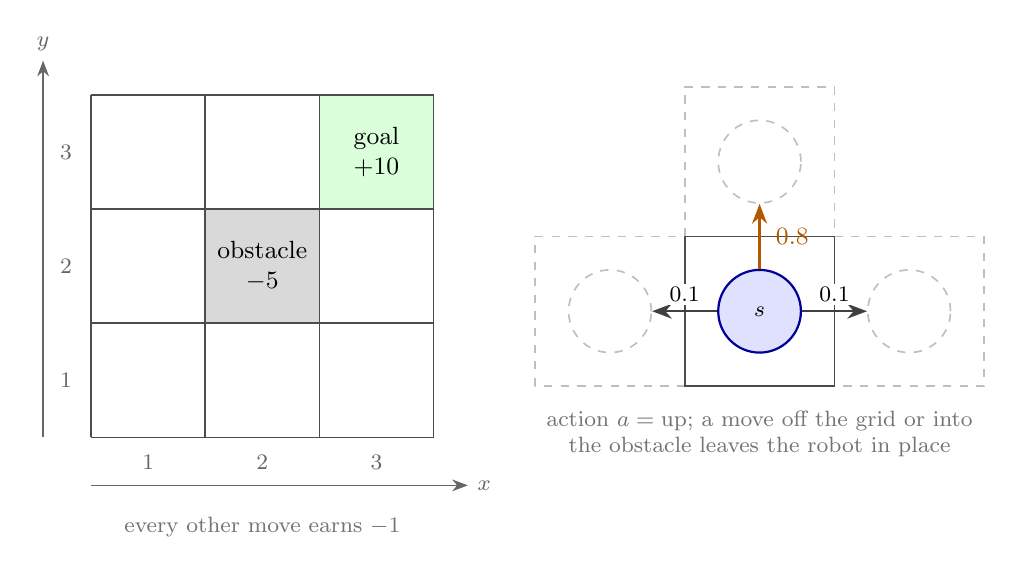
\begin{tikzpicture}[x=1.45cm,y=1.45cm]
  % --- Grid world: cell (x,y) spans (x-1,y-1) to (x,y) ---
  \fill[green!14] (2,2) rectangle (3,3);
  \fill[gray!30]  (1,1) rectangle (2,2);
  \foreach \i in {0,...,3} \draw[black!70,line width=0.6pt] (\i,0) -- (\i,3) (0,\i) -- (3,\i);
  \node[align=center] at (2.5,2.5) {goal\\$+10$};
  \node[align=center] at (1.5,1.5) {obstacle\\$-5$};

  \draw[axis] (0,-0.42) -- (3.3,-0.42) node[right,tick] {$x$};
  \draw[axis] (-0.42,0) -- (-0.42,3.3) node[above,tick] {$y$};
  \foreach \i in {1,2,3} {
    \node[tick] at (\i-0.5,-0.22) {$\i$};
    \node[tick] at (-0.22,\i-0.5) {$\i$};
  }
  \node[note] at (1.5,-0.78) {every other move earns $-1$};

  % --- Slip model for the action up ---
  \begin{scope}[shift={(5.2,0.45)},x=1.9cm,y=1.9cm]
    \draw[neighbor] (0,1) rectangle (1,2);
    \draw[neighbor] (-1,0) rectangle (0,1);
    \draw[neighbor] (1,0) rectangle (2,1);
    \draw[cell] (0,0) rectangle (1,1);
    \node[state] (r) at (0.5,0.5) {$s$};
    \node[state,draw=gray!50,fill=none,dashed,line width=0.6pt] (gu) at (0.5,1.5) {};
    \node[state,draw=gray!50,fill=none,dashed,line width=0.6pt] (gl) at (-0.5,0.5) {};
    \node[state,draw=gray!50,fill=none,dashed,line width=0.6pt] (gr) at (1.5,0.5) {};
    \draw[chosen] (r) -- (gu) node[midway,right=2pt,text=orange!70!black] {$0.8$};
    \draw[arr] (r) -- (gl) node[prob,midway,above=2pt] {$0.1$};
    \draw[arr] (r) -- (gr) node[prob,midway,above=2pt] {$0.1$};
    \node[note,align=center] at (0.5,-0.32)
      {action $a=\text{up}$; a move off the grid or into\\the obstacle leaves the robot in place};
  \end{scope}
\end{tikzpicture}
\end{document}
